\scanpage{411}
\mspage{208}

et sauf erreur, il est devenu évident
que ce foncteur est une \uline{équivalence de
catégories} (et comme \unsure{conséquence}, il
\margin{\illegible{1} \unsure{pour} \uline{$\unsure{i_0|i_\nu}$}}
y a le foncteur en sens inverse :
\unsure{forer} des trous en des ``pts'' invariants
sous $\Gamma_{\unsure{a|0}}$ (ou en des pts quelconques
quitte à passer à un $\Gamma'$ plus petit).

Mais je me rends compte que
\deleted{\illegible{1}} ce n'est pas du tout évident -- je vais
essayer d'élucider la situation axiomatiquement.
On a fixé un genre $g$,
on suppose donné, pour $\nu$ variable
(tel que $(g,\nu)$ anabélien) des
sous-groupes fermés $N_{g,\nu}\subset\unsure{\widehat{\widehat{\mathcal T}}_{g,\nu}}$,
normalisant $\unsure{\widehat{\mathcal T}_{g,\nu}}$, et satisfaisant la
condition essentielle que les $\psi:\unsure{\widehat{\widehat{\mathcal T}}_{g,\nu}}\longrightarrow\unsure{\widehat{\widehat{\mathcal C}}_{g,\nu-1}}$
\unsure{induisent|induisant}
\[
\unsure{N_{g,\nu}|M_{g,\nu}}\xrightarrow{\sim}\unsure{N_{g,\nu-1}|M_{g,\nu-1}}
\]
Ce qui permet de définir la notion
d'arithmétisation d'un $\pi$ profini de
type $(g,\nu)$ anabélien, et la théorie du

\scanpage{412}

bouchage d'un \unsure{nb} quelconque de trous, et
du forage d'1 seul trou, dans la
catégorie des groupes de type $g,\nu$,
arithmétisés.

On suppose d'autre part \unsure{donné|donnée} une
sous-catégorie pleine de la cat. des groupes
\margin{\illegible{3} : stable par prise des ss-groupes ouverts.}
profinis (qui pourrait se réduire aux
sous-groupes ouverts de $\unsure{\Pi_g}$, ou bien
\illegible{1} des $\Pi_{g,\nu}$ par des sous-groupes
ouverts des groupes $\Gamma_{\unsure{a|0}}$, avec
arithmétisation), et \deleted{des} \inserted{une notion d'}opérations
extérieures \inserted{\uline{``admissibles''}} de tels $\Gamma$ sur les
$\pi$ arithmétisés. On suppose

\textcircled{1} Si $\Gamma$ opère admissiblement sur $\pi$, \unsure{tt|$\forall$}
sous-groupe ouvert aussi (\deleted{\unsure{et}} et inversement ?)

\textcircled{2} Si de plus $\Gamma$ \unsure{invarie} une partie $I'$
\unsure{de} $I=I(\pi)$, alors en ``bouchant $I'$'',
l'opération de $\Gamma$ sur $\pi'$ est admissible.

\margin{Il suffit de le \unsure{prouver|poser} pour \unsure{$\operatorname{card} I'=1$}, i.e. \unsure{bouchage d'un seul} \uline{trou} -- \unsure{du moment qu'on sait que la condition d'admissibilité de l'action} \illegible{5}.}

\deleted{\illegible{1}}
\deleted{\unsure{On se propose de définir une notion d'action admissible} \illegible{2}}
\inserted{Quand on a une action \inserted{\uline{effective}}, \unsure{(non extérieure)}}
de $\Gamma$ sur un $(\pi,a)$, alors le foncteur
\unsure{de} ``\deleted{bouchage}\inserted{\unsure{forage}} des trous'' donne une action
ext. sur un $(\pi^0,a^0)$ de type $g,\nu+1$,
et on dit que l'action de départ est

\scanpage{413}
\mspage{209}

admissible, si l'action \uline{extérieure} déduite l'est.

On trouve ainsi une \uline{équivalence} entre
la cat. des \deleted{\unsure{cat.}} systèmes $(\pi,a,\Gamma,\psi,i)$
d'un $(\pi,a)$ de type $(g,\nu+1)$, avec une
op. \inserted{\uline{ext.}} admissible $\psi$ d'un $\Gamma$ dessus, et
un $i\in I(\pi)$ stable par $\Gamma$, avec la cat.
des $(\pi',a',\Gamma,\psi')$ des $(\pi',a')$ de type
$(g,\nu)$, avec une \uline{vraie} action admissible $\unsure{\psi'}$
de $\Gamma$ dessus.

\deleted{\unsure{On doit} \illegible{3}}
\inserted{La condition (1) \unsure{assure} que}
\deleted{\textcircled{3} \unsure{Si une vraie action}}
\inserted{si $\Gamma$ opère \deleted{\uline{\unsure{vraiment}}} \deleted{\unsure{admissible|admissiblement}} effectivement, de façon}
admissible, alors l'action extérieure déduite
est admissible (mais l'inverse ne
sera pas vrai -- il y aura des relèvements
``pathologiques'' d'une action ext. admissible
donnée). On suppose de plus

\margin{\figure{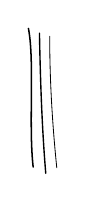
\begin{tikzpicture}[x=1cm,y=1cm,line cap=round,baseline=(current bounding box.center)]
\draw[line width=0.55pt] (0.04,1.80) .. controls (0.12,1.38) and (0.04,0.57) .. (0.10,0.04);
\draw[line width=0.50pt] (0.18,1.74) .. controls (0.19,1.20) and (0.21,0.55) .. (0.26,-0.04);
\draw[line width=0.30pt] (0.31,1.70) .. controls (0.31,1.09) and (0.35,0.52) .. (0.40,0.03);
\end{tikzpicture}}}
\textcircled{3} Si $\Gamma$ opère \inserted{effect.} de façon admissible sur
$\pi$, alors $\pi^\Gamma=(1)$.

\deleted{Soit \unsure{alors}}
Cela implique que la catégorie des
$\Gamma$-Pts \unsure{des|de} $\pi$, ou si on veut des sections
de $B_{\pi,\Gamma}\,(\unsure{\simeq}B_{\unsure{u|\mu}})$ sur $B_\Gamma$, est \uline{rigide}.

\scanpage{414}

Mais \deleted{\unsure{supposons}} considérons la catégorie limite inductive des \deleted{\illegible{1}} catégories des sections de $B_{\unsure{\pi|\Pi},\Gamma}\simeq \unsure{B_u}$ sur des $B_{\Gamma'}$ ($\Gamma'$ sous-groupe ouvert), elle est discrète et correspond à l'ens
\[
\mathrm{Pt}_{\mathrm{ad}}(B_{\unsure{\pi|\Pi},\unsure{\Gamma^{\natural}|\Gamma^{\flat}}})\simeq
\underset{\substack{\Gamma'\ \mathrm{ouvert}\\\mathrm{de}\ \Gamma}}{\varinjlim}
\mathrm{Pt}_{\mathrm{ad}}(B_{\unsure{\pi|\Pi},\Gamma'}).
\]

\margin{\uline{NB} Le \unsure{gr.-poïde} à \unsure{opérateurs stricts} $\uline{\mathrm{Pt}}(B_{\unsure{\pi|\Pi},\Gamma})$ dépend \unsure{fonctoriellement} de $(\unsure{\pi|\Pi},\Gamma)$, \illegible{1} pour des morphismes ext. \deleted{\unsure{dans}} \unsure{plus} \illegible{3} de $\Gamma$, si \deleted{\illegible{4}}.}

\deleted{\textcircled{4} \unsure{Pour} \illegible{2} $\mathrm{Pt}(B_{\unsure{\pi|\Pi},\Gamma})$ \illegible{1}. D'autre part, $\unsure{\pi|\Pi}$ peut être défini par un groupoïde.}
Si $\mathrm{Pt}(B_{\unsure{\pi|\Pi},\Gamma})\ne\varnothing$, alors (du seul fait que $\unsure{\pi|\Pi}^{\Gamma'}=(1)$ pour $\forall$ sous-groupe ouvert de $\Gamma$) \inserted{le gr. cat.} $\unsure{\pi|\Pi}$ peut être décrit \unsure{com.} par un groupoïde \inserted{profini $\uline{\mathrm{Pt}}(B_{\unsure{\pi|\Pi},\unsure{\Gamma^{\natural}|\Gamma^{\flat}}})$} ayant $\mathrm{Pt}(B_{\unsure{\pi|\Pi},\Gamma})$ comme ens d'objets, \deleted{alors} \inserted{\unsure{clifié} par le groupe cat. $\unsure{\pi|\Pi}$,} sur lequel $\Gamma$ opère au sens strict, avec \unsure{les stabilisateurs|le stabilisateur} $\Gamma_P$ de $\forall$ pt étant \unsure{ouverts|ouvert}. et $\Gamma_P\to\mathrm{Aut}(P)$ $(\unsure{\simeq\unsure{\pi|\Pi}_P},\ \unsure{\text{mod. autom. int.}})$

\deleted{De façon plus précise, \unsure{indépendamment de} l'axiomatique précédente, on peut décrire les syst. \unsure{formés} d'un groupe \inserted{cat. $\unsure{\pi|\Pi}$} profini, et d'une opération \inserted{ext.} \unsure{d'un groupe profini} $\Gamma$ dessus, \unsure{satisfaisant}}

étant continue. On a ici \unsure{par déf.} : $\forall\ P\in\mathrm{Pt}(B_{\unsure{\pi|\Pi},\Gamma})$ on associe la classe d'isom. de \deleted{\unsure{groupes de relèvements}}

\scanpage{415}
\mspage{210}

\deleted{\unsure{groupes}} \unsure{de|des} sections de $B_{\unsure{\pi|\Pi},\Gamma}$ sur $B_\Gamma$, on trouve une bijection -- ce qui caractérise le \inserted{$\Gamma$-}groupoïde en question à \uline{isom} unique près. On suppose

\textcircled{4} Si $\Gamma$ opère admissiblement sur $(\unsure{\pi|\Pi},a)$, alors il existe un sous-groupe ouvert $\Gamma'$ de $\Gamma$ \deleted{peut \unsure{opérer de façon}} \inserted{dont l'op. \inserted{cat.} \unsure{se relève} en une} op. effective admissible -- i.e. $\mathrm{Pt}_{\mathrm{ad}}(B_{\Gamma,\unsure{\pi|\Pi}})\ne\varnothing$.

\deleted{Ceci dit, considérons \unsure{la} situation d'une action \inserted{ext.} admissible de $\Gamma$ sur $(\unsure{\pi|\Pi},a)$ et d'un $i\in I(\unsure{\pi|\Pi})$ \deleted{stable} fixe sous $\Gamma$. On a donc une action \uline{effective} \inserted{\unsure{admiss.}} de $\Gamma$ sur $(\unsure{\pi|\Pi}',a')$, \deleted{et de plus on a} \inserted{donc une action extérieure,} plus un Pt ``$\Gamma$-rationnel'', i.e. invariant sous $\Gamma$. Considérons d'autre part un \unsure{relèvement} admissible $\Gamma\longrightarrow M(\unsure{\pi|\Pi},a)$, et \illegible{2}}

Notons que dans la situation envisagée, du bouchage d'un trou $i\in I(\unsure{\pi|\Pi})$ d'un $\unsure{\pi|\Pi}$, en plus de l'hom.
\[
\unsure{\widehat{\widehat{\mathcal T}}}(\unsure{\pi|\Pi})_i
\xrightarrow{\psi_i}
\unsure{\widehat{\widehat{\mathcal C}}}(\unsure{\pi|\Pi}'_i)
\]
\unsure{on a ici|on a aussi}, donnant par composition
\[
\unsure{\widehat{\widehat{\mathcal T}}}(\unsure{\pi|\Pi})_i
\xrightarrow{\psi'_i}
\unsure{\widehat{\widehat{\mathcal T}}}(\unsure{\pi|\Pi}'_i)
\]

\scanpage{416}

d'où une action extérieure de $\unsure{\widehat{\widehat{\mathcal T}}}(\unsure{\pi|\Pi})$ sur $\unsure{\pi|\Pi}'_i$, \deleted{\illegible{3}} \inserted{\deleted{\illegible{1}} $\unsure{\pi|\Pi}\overset{p_i}{\longrightarrow}\unsure{\pi|\Pi}'_i$ comme \unsure{morph. act. ext.|morph. équ. ext.} de $\unsure{\widehat{\widehat{\mathcal T}}}(\unsure{\pi|\Pi})$, \deleted{\illegible{1}}} on a un homomorphisme canonique d'extensions, \deleted{\unsure{associé}} provenant de cette action extérieure et de l'hom. $p_i:\unsure{\pi|\Pi}\longrightarrow\unsure{\pi|\Pi}'_i$,

\diagram{\begin{tikzcd}[ampersand replacement=\&,column sep=2.4em,row sep=3.4em,
execute at end picture={
  \path (\tikzcdmatrixname-1-4.south west) -- (\tikzcdmatrixname-2-3.north east) coordinate[pos=.5] (lmfixnineteendiag);
  \draw[line width=.35pt] ([xshift=-5mm,yshift=1mm]lmfixnineteendiag) -- ([xshift=-6mm,yshift=1mm]lmfixnineteendiag) -- ([xshift=-6mm,yshift=-5mm]lmfixnineteendiag) -- ([xshift=-5mm,yshift=-5mm]lmfixnineteendiag);
  \draw[line width=.35pt] ([xshift=8mm,yshift=5mm]lmfixnineteendiag) -- ([xshift=9mm,yshift=5mm]lmfixnineteendiag) -- ([xshift=9mm,yshift=-1mm]lmfixnineteendiag) -- ([xshift=8mm,yshift=-1mm]lmfixnineteendiag);
}]
1 \arrow[r,dash] \& \pi \arrow[r,dash] \arrow[d,"\unsure{p_i}"] \&
\widehat{\widehat{\unsure{\mathcal G}}}(\pi)_i \arrow[r] \arrow[d,"\varphi_i"] \&
\widehat{\widehat{\mathcal T}}(\pi)_i \arrow[r,dash] \arrow[d,"\psi'_i"] \arrow[dl,dashed,"\psi_i"'] \& 1 \\
1 \arrow[r,dash] \& \pi'_i \arrow[r] \&
\widehat{\widehat{\unsure{\mathcal G}}}(\pi'_i) \arrow[r,dash] \&
\widehat{\widehat{\mathcal T}}(\pi'_i) \arrow[r,dash] \& 1
\end{tikzcd}}

qui vient par la composée
\[
\unsure{\widehat{\widehat{\mathcal C}}}(\unsure{\pi|\Pi})_i
\longrightarrow\unsure{\widehat{\widehat{\mathcal T}}}(\unsure{\pi|\Pi})_i
\xrightarrow{\psi_i}\unsure{\widehat{\widehat{\mathcal C}}}(\unsure{\pi|\Pi}'_i).
\]
(il peut se définir chaque fois qu'on a un groupe $\Gamma$, ici $\unsure{\widehat{\widehat{\mathcal T}}}(\unsure{\pi|\Pi})$, qui \unsure{opérant|opère} extérieurement sur deux groupes cat. $\unsure{\pi|\Pi},\unsure{\pi|\Pi}'$, \deleted{de centre trivial} et qu'on a un hom \inserted{\unsure{ext.}} $\unsure{\beta}:\unsure{\pi|\Pi}\longrightarrow\unsure{\pi|\Pi}'$ qui commute à l'action de $\Gamma$, et tel que le \inserted{centre de $\unsure{\pi|\Pi}$ et \unsure{le|les}} \unsure{centralisateur|centralisateurs} de \unsure{$\beta(\unsure{\pi|\Pi})$} dans $\unsure{\pi|\Pi}'$ soient triviaux\ldots)
\inserted{\unsure{C'est} \illegible{1} l'hom de ``\unsure{transport de str.}''}, $\unsure{\beta_0}$ \inserted{qui} \unsure{à} \unsure{\deleted{tout}} \unsure{autom.} à droite $u$ de $\unsure{\pi|\Pi}$, associe l'autom. \unsure{canonq.|conj.} de $\unsure{\pi|\Pi}'_i$.

On \deleted{\unsure{avait}} oublié de préciser :

\textcircled{\unsure{7|2}} L'hom canonique $(\unsure{\widehat{\widehat{\mathcal C}}}_{g,\nu})_i\longrightarrow\unsure{\widehat{\widehat{\mathcal C}}}_{g,\nu-1}$ associé à $i\in[0,\nu-1]$, envoie $(M_{g,\nu})_i$ dans $M_{g,\nu-1}$ \deleted{dans} donc il s'insère dans un \unsure{diagr.} de suites exactes

\scanpage{417}
\mspage{211}

(26)
\diagram{
\begin{tikzcd}[ampersand replacement=\&]
1 \arrow[r,dash] \& \pi \arrow[r,dash] \arrow[d] \&
\unsure{M_{\unsure{a|c}}(\pi)_i} \arrow[r] \arrow[d, "\varphi_i"']
\arrow[dr, phantom, "{\text{\unsure{\uline{non}|\uline{pas}} \unsure{comm.?}}}" description, near start] \&
N_{\unsure{a|c}}(\pi)_i \arrow[r] \arrow[d] \arrow[dl, dashed, "\text{\unsure{canon.}}"'] \& 1 \\
1 \arrow[r,dash] \& \pi'_i \arrow[r] \&
M_{\unsure{a'|c'}}(\pi'_i) \arrow[r,dash] \& N_{\unsure{a'|c'}}(\pi'_i) \arrow[r,dash] \& 1
\end{tikzcd}
\par [Les segments horizontaux issus des deux $1$ de gauche n'ont pas de pointe visible. Les extrémités droites des segments $\pi$--$M_{\unsure{a|c}}(\pi)_i$ en haut, $M_{\unsure{a'|c'}}(\pi'_i)$--$N_{\unsure{a'|c'}}(\pi'_i)$ et $N_{\unsure{a'|c'}}(\pi'_i)$--$1$ en bas sont épaissies, sans pointe lisible avec certitude.]
}.

Ceci posé, si on a une opération \inserted{ext} admissible
$\Gamma\longrightarrow N_{\unsure{a|c}}(\pi)$ de $\Gamma$ sur $\pi$,
\inserted{fixant $i$,} \unsure{donc} aussi par
$N_{\unsure{a|c}}(\pi)\longrightarrow N_{\unsure{a'|c'}}(\pi'_i)$ sur $\pi'_i$,
on peut considérer que \unsure{\deleted{tout}} relèvement
$\Gamma\longrightarrow M_{\unsure{a|c}}(\pi)$ \inserted{pour $\pi$} définit
par composition un relèvement $\Gamma\longrightarrow M_{\unsure{a'|c'}}(\pi'_i)$
pour $\pi'_i$. \deleted{Dire que}
\inserted{On \unsure{conclut} \unsure{aisément} de}
\textcircled{2} que si le premier est admissible, le deuxième l'est.
On trouve donc
\[
(27)\qquad
\mathrm{Pt}_{\mathrm{ad}}(B_{\pi,\Gamma})
\longrightarrow
\mathrm{Pt}_{\mathrm{ad}}(B_{\pi'_i,\Gamma})
\]
(et en passant à la limite, une application de $\Gamma$-ensembles
\[
(28)\qquad
\mathrm{Pt}_{\mathrm{ad}}(B_{\pi,\unsure{\Gamma^{\natural}|\Gamma^{\flat}}})
\longrightarrow
\mathrm{Pt}_{\mathrm{ad}}(B_{\pi'_i,\unsure{\Gamma^{\natural}|\Gamma^{\flat}}})
\]
-- qui correspond d'ailleurs à un hom. de \unsure{$\Gamma$} groupoïdes
\[
(29)\qquad
\uline{\mathrm{Pt}}_{\mathrm{ad}}(B_{\pi,\unsure{\Gamma^{\natural}|\Gamma^{\flat}}})
\longrightarrow
\uline{\mathrm{Pt}}_{\mathrm{ad}}(B_{\pi'_i,\unsure{\Gamma^{\natural}|\Gamma^{\flat}}}).
\]

Ceci posé, soit $P\in\mathrm{Pt}_{\mathrm{ad}}(B_{\pi'_i,\Gamma})$
le ``pt canonique'' de
$\mathrm{Pt}_{\mathrm{ad}}B_{\pi'_i,\Gamma}
=\bigl(\mathrm{Pt}_{\mathrm{ad}}(B_{\pi'_i,\unsure{\Gamma^{\natural}|\Gamma^{\flat}}})\bigr)^\Gamma$.

\scanpage{418}

On demande :

\textcircled{5} L'application (27) induit une \uline{bijection}\unsure{.}
\figure{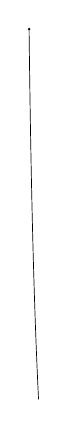
\begin{tikzpicture}[x=1mm,y=1mm,baseline=(current bounding box.north)]
\fill (0,0) circle[radius=.18mm];
\draw[line width=.25pt,line cap=round] (0,-.2) .. controls (.15,-13) and (.45,-32) .. (1.2,-47);
\end{tikzpicture}}
\[
\mathrm{Pt}_{\mathrm{ad}}(B_{\pi,\Gamma})
\longrightarrow
\mathrm{Pt}_{\mathrm{ad}}(B_{\pi'_i,\Gamma})\setminus\{P\}
\]
ou encore (\unsure{passant} à la limite) une bijection de $\Gamma$-ensembles
\[
\mathrm{Pt}_{\mathrm{ad}}(B_{\pi,\unsure{\Gamma^{\natural}|\Gamma^{\flat}}})
\simeq
\mathrm{Pt}_{\mathrm{ad}}(B_{\pi'_i,\unsure{\Gamma^{\natural}|\Gamma^{\flat}}})\setminus\{P\}
\]

Ceci signifie trois choses :

a) L'hom canonique $\Gamma\longrightarrow M_{a'}(\pi'_i)$,
composé de $\Gamma\longrightarrow N_a(\pi)$ et de
$N_a(\pi)\simeq M_{a'}(\pi'_i)$,
n'est pas \inserted{$\pi'_i$-}conjugué à un hom composé
$\Gamma\xrightarrow{\lambda}M_a(\pi)
\xrightarrow{\varphi_i}M_{a'}(\pi'_i)$,
où $\Gamma\xrightarrow{\lambda}M_a(\pi)$ est un relèvement admissible.

b) Si $\lambda,\mu:\Gamma\rightrightarrows M_a(\pi)$ sont deux
relèvements admissibles de $\Gamma\longrightarrow N_a(\pi)$
\deleted{\unsure{que}} tels que
$\varphi_i\circ\lambda$ et $\varphi_i\circ\mu:
\Gamma\rightrightarrows M_a(\pi)$ soient
\inserted{$\pi'_i$-}conjugués, alors $\lambda$ et $\mu$ sont déjà
\inserted{$\pi$-}conjugués.

c) Tout relèvement admissible de
$\Gamma\longrightarrow N_{a'}(\pi'_i)$ en
$\Gamma\longrightarrow \unsure{M_{a'}(\pi'_i)}$,
provient par composition d'un rel. admissible
$\Gamma\longrightarrow M_a(\pi)$.

\scanpage{419}
\mspage{212}

\unsure{Grâce} à ceci, l'équivalence de catégories entre systèmes
$(\pi,a,i,\Gamma,\unsure{\theta}:\Gamma\mathop{\longrightarrow}\limits_{\unsure{\mathrm{adm}}}\unsure{N_a})$,
et les systèmes $(\pi',a',\Gamma,\theta':\Gamma\longrightarrow\unsure{N_{a'}},P)$,
où $P\in\mathrm{Pt}(B_{\pi',\unsure{\Gamma^{\natural}|\Gamma^{\flat}}})^\Gamma$,
se précise de façon \unsure{parfaite} au niveau des points: les
Points $\Gamma$-rationnels de $B_{\unsure{\pi,\Gamma^{\natural}|\pi,\Gamma^{\flat}}}$
s'identifient à \unsure{l'ens}
\deleted{des pts $\Gamma$-\unsure{rationnels}} des pts $\Gamma$-rationnels
de $B_{\pi'}$, distincts de $P$.

Ceci nous permet alors (ce qui n'était pas faisable dans le \unsure{contexte}
discret!) d'étendre l'équivalence de catégories en une équivalence

\[
(30)\qquad
\begin{array}{c@{\quad}c@{\quad}c}
\parbox[t]{0.45\linewidth}{%
cat. des systèmes $(\pi,a,I',\Gamma,\theta:\Gamma\longrightarrow N_a)$
d'un $\pi$ arithmétisé \inserted{\unsure{(par $a$)}} de type $(g,\nu)$,
de $I'\subset I(\pi)$, d'une action
\uline{admissible} ext. de $\Gamma$ sur $\pi$
telle que $\Gamma$ \deleted{\unsure{op.}} \uline{fixe chaque point} de $I'$
}
& \unsure{\cong|\simeq} &
\parbox[t]{0.36\linewidth}{%
cat des syst.
$(\pi',\unsure{a'|\alpha'},I',\unsure{\Gamma^{*}|\Gamma},\theta':\Gamma\longrightarrow N_{a'})$
d'un $\pi'$ arithmétisé (par \unsure{$a'$|$\alpha'$}) de type
$(g,\nu')$ $[\nu'=\nu-\mathrm{card}(I')]$
avec op. \inserted{ext.} admissible de $\Gamma$ dessus, et
une partie $I'\subset\mathrm{Pt}_{ad}(B_{\pi',\unsure{\Gamma}}\unsure{)}$
(donc $I'\subset\mathrm{Pt}_{ad}(B_{\pi',\Gamma})^\Gamma$)
i.e. $I'$ formé de pts \unsure{fixes} par $\Gamma$, i.e. ``$\Gamma$-rationnels''
}
\end{array}
\]

\margin{avec $2g+(\underbrace{\nu-\mathrm{card}\,I'}_{\nu'})\geq3$}

On a donc un foncteur quasi-inverse:
\unsure{forage} de trous en $I'$ !

\scanpage{420}

Il est à noter que dans cette approche, on a dû se borner au cas
\deleted{\unsure{des|de}} \inserted{d'un ens de} pts \deleted{\illegible{1}}
$I'\subset I(\pi)$ non seulement stable par $\Gamma$, mais
\deleted{\unsure{formé}} $\subset I^\Gamma$
\deleted{fixes par $\Gamma$} ou encore à une partie
$I'\subset\mathrm{Pt}(B_{\pi',\unsure{\Gamma^{\natural}|\Gamma^{\flat}}})$
non seulement stable par $\Gamma$, mais
$\unsure{I'|=}\subset\mathrm{Pt}(B_{\pi',\unsure{\Gamma^{\natural}|\Gamma^{\flat}}})^\Gamma$.
Pour montrer que sans cette restriction, le foncteur naturel
\deleted{\unsure{est}} \unsure{correspondant} est \unsure{néanmoins}
une équivalence, on est ramené à ceci

\textcircled{6} Soit $(\pi,a,I'\subset I(\pi))$ avec $(\pi,a)$
\unsure{groupoïde} \inserted{\unsure{cat.}} \unsure{profini|profi.} arithmétisé de type
$g,\nu$, \unsure{d'où} $(\pi',a')$ --- soit $\Gamma$, avec $\Gamma'$
sous-groupe ouvert opérant sur $(\pi,a)$ de façon admissible
$(\unsure{\Gamma|\Gamma'}\longrightarrow N_a(\pi))$,
et laissant stable $I'$, donc il \unsure{opère} de façon admissible sur
$(\pi',a')$,
Supposons donné un \uline{relèvement} de cette action de $\Gamma'$
en une action admissible de $\Gamma$ sur $N_{a'}$, qui \unsure{invarie}
\[
\begin{array}{rcl}
I'&\subset&\mathrm{Pt}(B_{\pi',\unsure{\Gamma^{\natural}|\Gamma^{\flat}}}).\\
&&\rotatebox{90}{$\unsure{\simeq}$}\\
&&\mathrm{Pt}(B_{\pi',\unsure{\Gamma^{\prime\natural}|\Gamma^{\prime\flat}}})
\end{array}
\]

\diagram{\begin{tikzcd}[ampersand replacement=\&,column sep=3.6em,row sep=3em]
{\deleted{\unsure{M_a}}\;(N_a)_{I'}} \arrow[d] \&
\Gamma' \arrow[l] \arrow[d,hook,line width=.9pt] \arrow[dl,bend right=7,line width=.65pt] \\
N_{a'} \& \Gamma \arrow[l] \arrow[ul,dashed]
\end{tikzcd}}

Alors il existe une action admissible unique de $\unsure{\Gamma|\Gamma'}$
sur $(\pi,a)$, qui prolonge celle de $\Gamma'$ et qui donne naissance
à celle \inserted{donnée} sur $\pi'$.
